% Lecture Template for ME3001-001-Tristan Hill - Spring 2017
% 
% Mechanical Engineering Analysis with MATLAB
%
% Roots of Non- Linear Equations - Lecture 2

% Document settings
\documentclass[11pt]{article}
\usepackage[margin=1in]{geometry}
\usepackage[pdftex]{graphicx}
\usepackage{multirow}
\usepackage{setspace}
\usepackage{hyperref}
\usepackage{color,soul}
\usepackage{fancyvrb}
\usepackage{framed}
\usepackage{wasysym}
\usepackage{multicol}

\pagestyle{plain}
\setlength\parindent{0pt}
\hypersetup{
    bookmarks=true,         % show bookmarks bar?
    unicode=false,          % non-Latin characters in Acrobat’s bookmarks
    pdftoolbar=true,        % show Acrobat’s toolbar?
    pdfmenubar=true,        % show Acrobat’s menu?
    pdffitwindow=false,     % window fit to page when opened
    pdfstartview={FitH},    % fits the width of the page to the window
    pdftitle={My title},    % title
    pdfauthor={Author},     % author
    pdfsubject={Subject},   % subject of the document
    pdfcreator={Creator},   % creator of the document
    pdfproducer={Producer}, % producer of the document
    pdfkeywords={keyword1} {key2} {key3}, % list of keywords
    pdfnewwindow=true,      % links in new window
    colorlinks=true,       % false: boxed links; true: colored links
    linkcolor=red,          % color of internal links (change box color with linkbordercolor)
    citecolor=green,        % color of links to bibliography
    filecolor=magenta,      % color of file links
    urlcolor=blue           % color of external links
}

% assignment number 
\newcommand{\NUM}{2} 
\newcommand{\VSpaceSize}{2mm} 
\newcommand{\HSpaceSize}{2mm} 

\definecolor{mygray}{rgb}{.6, .6, .6}

\setulcolor{red} 
\setstcolor{green} 
\sethlcolor{mygray} 

\begin{document}

\textbf{ \LARGE ME 3001 Lecture, Roots of Non-Linear Equations} \\

\begin{itemize}


	\item \textbf{ \LARGE Theoretical/Analytical Solution Techniques }
			\begin{itemize}
				\item \LARGE{solving the equation using exact mathematics} \\
				\item \LARGE{leads to an exact or {\it analytical} solution} \\ \vspace{40mm}
				
			\end{itemize}
	\item \textbf{ \LARGE Numerical Solution Techniques }		
			\begin{itemize}
				\item \LARGE{ approximating the solution to the equation using varying methods, or {\it algorithms} } \\
				\item \LARGE{leads to a approximate solution} \\ 
				\item \LARGE{a.k.a. {\it Numerical Method}}\vspace{20mm}
			\end{itemize}
\newpage

	\item \textbf{ \LARGE Method 3 - {\it Newton -Raphson Method}}
		\begin{itemize}
			\item \LARGE{Isaac Newton, mathematician and physicist, 1642-1727}
			\item \LARGE{Joseph Raphson, English Mathematician, 1648-1715} \\\\
			\item \LARGE{Taylor Series Derivation:} \\
		

				\scalebox{1}{$f(x)\approx f(a)+f'(a)(x-a)+\frac{f''(a)}{2!}(x-a)^2+...+\frac{f^{(n)}(a)}{n!}(x-a)^{(n)}$} \vspace{50mm}
		
\newpage

		\item \LARGE{Graphical Explanation:} \\\\
		
\includegraphics[scale=.5]{lecture2_fig1.png}\\
		\item \LARGE{Slope Triangle:} \\
		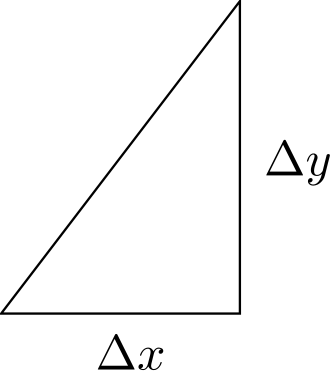
\includegraphics[scale=.5]{lecture2_fig2.png}
		
		\newpage
		\item \LARGE{sign is handled !} \\\\
		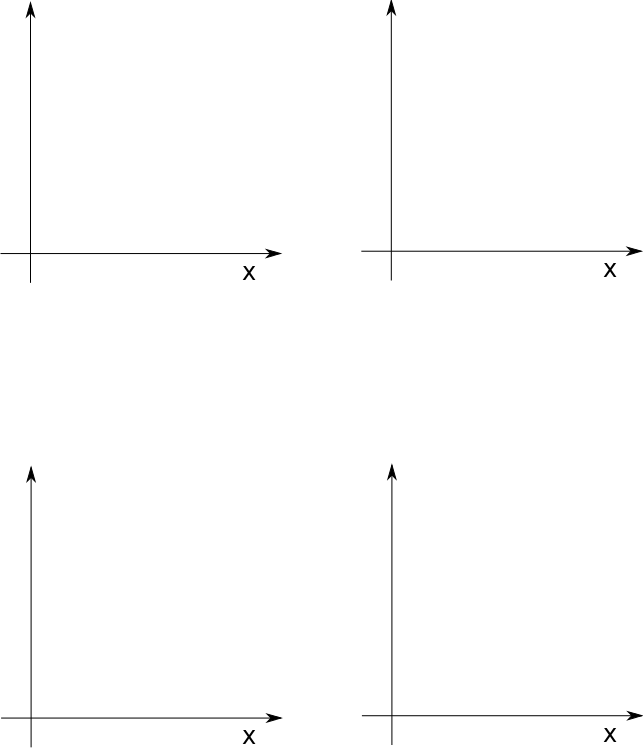
\includegraphics[scale=.7]{lecture2_fig4.png}
		
		\newpage
	
		\item \LARGE{Issues with the {\it Newton - Raphson} Method} \\\\
		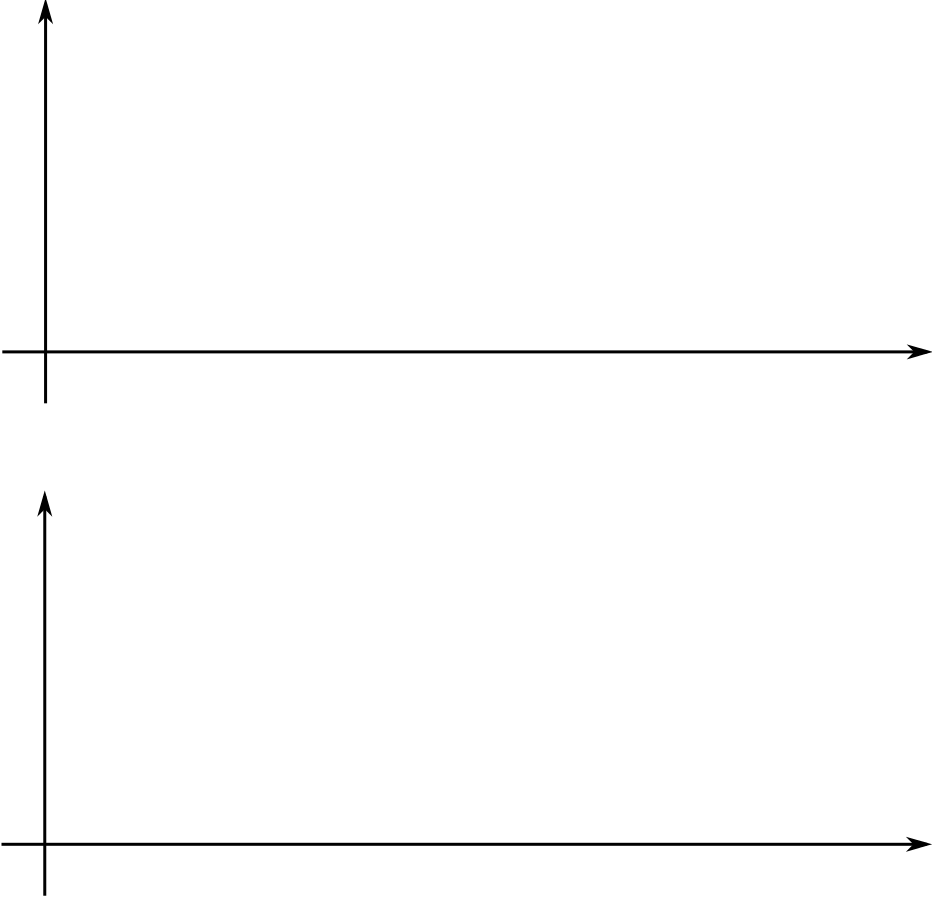
\includegraphics[scale=.5]{lecture2_fig5.png}

		\end{itemize}
\newpage

	\item \textbf{ \LARGE Method 4 - {\it Secant Method (modified Newton-Raphson)}}
\begin{itemize}	
	\item \LARGE{Forward Difference}\\
	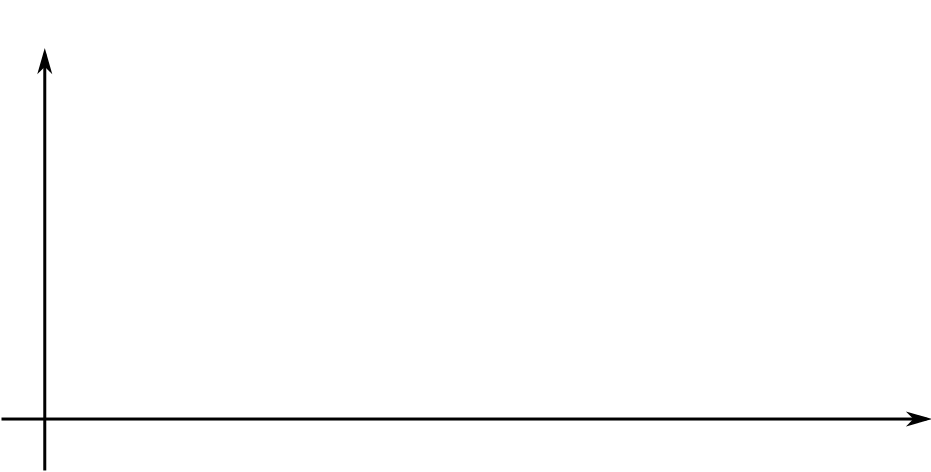
\includegraphics[scale=.35]{lecture2_fig6.png}\\
	\item \LARGE{Backwards Difference}\\
	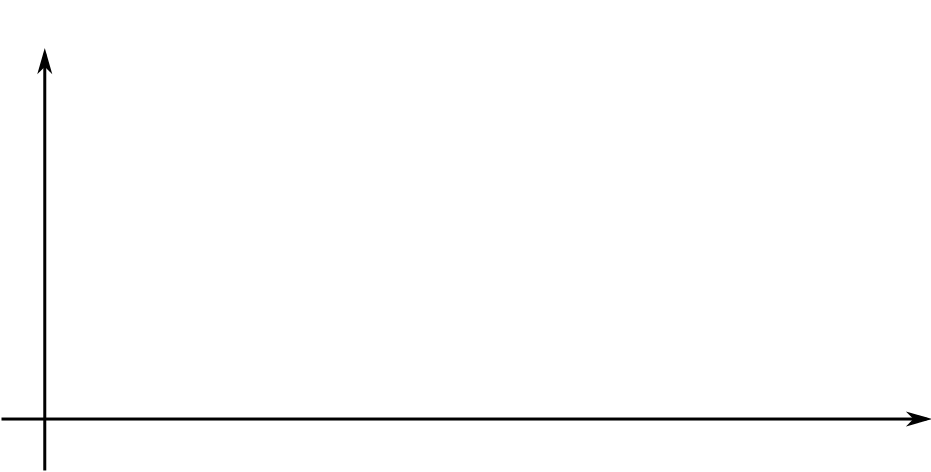
\includegraphics[scale=.35]{lecture2_fig6.png}\\
	\item \LARGE{Central Difference}\\
	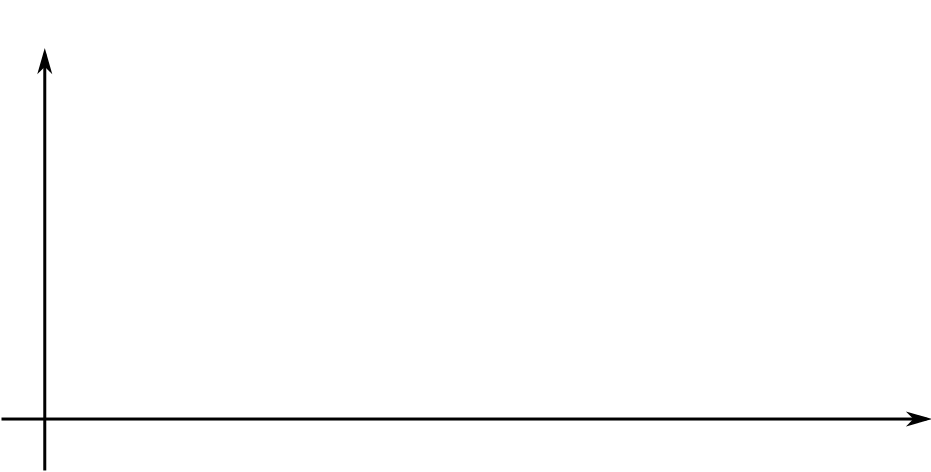
\includegraphics[scale=.35]{lecture2_fig6.png}
\newpage
	\item \LARGE{These are know as {\it Finite Difference Approximations} }\\
	\item \LARGE{When used in the {\it Newton-Raphson} equation this becomes the {\it Secant Method} }\\
		
		
\end{itemize}

\newpage 

	\item \textbf{ \LARGE REMINDER - Homework 1 is due Friday } \\
	 
	\item \textbf{ \LARGE REMINDER - MATLAB script from today's lecture will be posted on ilearn. } \\

\end{itemize}


	

\end{document}



